\documentclass[../main/Notes.tex]{subfiles}
\begin{document}

\section[Measuring Beliefs I]{Measuring Beliefs I \iftoggle{showdates}{\small{\textit{2014-05-02}}}{}}

% TODO: Someone has to think over this section and write some better text. This clearly is not enough.
\subsection{Probability as Belief}
We can measure probabilities for recurring events, how can we measure probabilities for unique events?

Unique events are for example:
\begin{itemize}
	\item How sure are people which population is bigger, the EU or the US population?
  \item How can bookmakers set the odds for soccer games?
  \item How high is the probability for a nuclear reactor to blow up?
\end{itemize}

The frequentist view is not really helpful here: Since those events don't appear numerous times, you can not measure any limits of relative frequencies. But the Bayesian view helps us to use the same math to determine these probabilities.

\subsection{What do you accept as a fair bet?}\index{Fair Bet}
\begin{figure}[ht]
  \begin{center}
    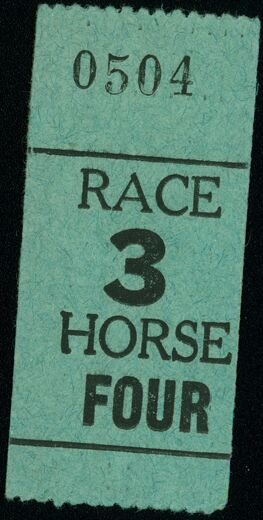
\includegraphics[]{../images/Oronsay-Rick-Danley-Horse-Race-ticket-June-30.jpg}
    \caption{A horse race ticket. \textit{Source: Reuben Goossens, ssmaritime.com}}
    \label{fig:raceticket}
  \end{center}
\end{figure}

Let's assume for the next examples that people are honest (Otherwise they would lie to win).

Assume you have a ticket you can exchange for \$1 if A happens, otherwise it's worth nothing.

\begin{align*}
Ticket = 
  \begin{cases}
    \$1 \mbox{ if } A \\
    \$0 \mbox{ else}
  \end{cases}
\end{align*}

What would be a fair price for that ticket?
\begin{align*}
\left(\$1 - c\right) P(A) - cP(\neg A) &= 0 \\
\Leftrightarrow P(A) &= c
\end{align*}

\subsubsection*{Coherence (fair pricing)}\index{Coherence}
\begin{enumerate}
	\item $P(certain) = 1$, $P(impossible) = 0$
  \item $\forall A\ 0 \leq P(A) \leq 1$
  \item $P(A \cap B) = \left\{\right\} \rightarrow P(A \cup B) = P(A) + P(B)$
\end{enumerate}

These rules follow from some logical thoughts.

Imagine $P(A) + P(\neg A) > 1$. Then the bookmaker would make money and the bet wasn't fair. If you are not the bookmaker, you want to have something like $P(A) + P(\neg A) < 1$.

Another case is $A \cap B = \left\{\right\}$, i.e. $A$ and $B$ are mutually exclusive. Then you want to buy $P(A)+P(B)$ but sell $P(A \cup B)$ if $P(A) + P(B) < P(A \cup B)$.

\subsection{Conditional Bets}
If we don't have repeatable events, how can we justify conditional probabilities\index{Conditional Probability}?

Assume a ticket again, this time of the following form:
\begin{align*}
Ticket = 
  \begin{cases}
    \$1 \mbox{ if } A \cap B \\
    \$c \mbox{ if } \neg B \mbox{\textit{(refund)}} \\
    \$0 \mbox{ else}
  \end{cases}
\end{align*}

A is dependent on B now.
% Here I also have 
% \begin{align*}
%   P(A|B) \mbox{ if }\neg B \\
%   P(\neg B) \cdot P(A|B)
% \end{align*}
% but I don't know how to explain it
\begin{align*}
P(A|B)     &=       P(A \cap B)          + P(\neg B) P(A|B) \\
         1 &= \frac{P(A \cap B)}{P(A|B)} + 1 - P(B)         \\
      P(B) &= \frac{P(A \cap B)}{P(A|B)}                    \\
P(A|B)P(B) &=       P(A \cap B)                             \\
P(A|B)     &= \frac{P(A \cap B)}{P(B)}
\end{align*}

\subsection*{Philosophical differences matter}
Alice has two coins, coin 1 with a probability of 0.5 for heads and tails, coin 2 with probability 0.4 for heads (and 0.6 for tails). 

She chooses a coin and tells Bob she would flip it $n$ times now. Then Bob has to guess which coin she flipped.

Bob has two hypotheses, one for each coin. To check his hypotheses, he can now use the data (i.e. the $n$ coin flips) and calculate the probabilities for his hypotheses - then he can compare those and choose the one with higher probability.
\begin{align*}
P(H|D) = \frac{P(D|H)P(H)}{P(D)}
\end{align*}
\textit{(with H = Hypothesis, D = Data)}

\subsection*{Calibration and Coherence}\index{Calibration}\index{Coherence}
\sidenote{In short: Being ill-\-ca\-li\-bra\-ted means you lose money on average, while being incoherent means you lose it.}
Note that there is a difference between coherence and calibration.
You are well calibrated if you answer according to your real beliefs and knowledge. For example if you play Roulette you do bet although you know that you can lose because of the 0, so you are not well calibrated (a well calibrated person in that case would not play). 
Being coherent means that you follow the rules of probability, for example that you don't trip into the conjunction fallacy trap\index{Conjunction Fallacy} (see the chapter about ``Conditional Bets'' above).

\end{document}